% ============================================================
\chapter{Black-Litterman の全体像：何をどこで決めるか}\label{ch:overview}

この章では、BL の計算の流れをたどり、決めなければならない値を一覧にする。そのうえで、この資料の中心になる「採用率」という見方を、1 資産・1 ビューの場合で導く。

\section{平均分散最適化の弱点と、BL の考え方}

平均分散最適化は、期待リターン $\mu$ と共分散 $\Sigma$ から、リスク回避度 $\delta$ のもとで
\begin{equation}
\max_w\; w\T\mu-\frac{\delta}{2}w\T\Sigma w
\label{eq:mvobj}
\end{equation}
を解く。制約がなければ答えは $w^*=(\delta\Sigma)^{-1}\mu$ である。この式は $\mu$ の小さな違いに非常に敏感で、過去の平均リターンを $\mu$ に入れると、極端な買いと売りが並ぶ比率になる。Idzorek（2007）の 8 資産の例では、過去 60 か月の平均を使うと、米国債券が 1144\%、外国債券が $-105\%$ という比率になる（\chapref{ch:idzorek}）。$\mu$ の推定の誤差が、最適化で増幅されるためである（Michaud 1989 の言う「誤差の最大化」）。

BL は、$\mu$ を直接推定しない。まず、いまの時価総額の比率 $\wmkt$ が式~\eqref{eq:mvobj} の答えになっていると仮定して、$\mu$ を逆算する。
\begin{equation}
\Pi=\delta\Sigma\wmkt
\label{eq:pi}
\end{equation}
これを均衡リターンと呼ぶ。$\Pi$ を最適化に入れれば、答えは $\wmkt$ に戻る。つまり、ビューがなければ市場の比率を持つ。そのうえで、投資家のビューを確信の度合いに応じて混ぜ、$\Pi$ を少しだけ動かす。動かした分だけ、比率が市場からずれる。

\section{計算の流れ}

\begin{figure}[htbp]
\centering
\adjustbox{max width=\linewidth}{%
\begin{tikzpicture}[node distance=6mm and 8mm]
\node[box=c3] (w) {時価総額の比率\\$\wmkt$};
\node[box=c3,right=of w] (pi) {均衡リターン\\$\Pi=\delta\Sigma\wmkt$};
\node[box=c3,above=5mm of pi] (sig) {共分散 $\Sigma$\\リスク回避度 $\delta$};
\node[box=c4,below=12mm of w] (src) {ビューの材料\\（分析・モデル・LLM）};
\node[box=c4,right=of src] (q) {ビュー $P$, $Q$\\不確かさ $\Omega$};
\node[box=c1,right=14mm of $(pi)!0.5!(q)$] (bl) {BL の事後\\$\muBL$、$M$\\（$\tau$ を使う）};
\node[box=c1,right=of bl] (opt) {最適化\\（制約・TE）};
\node[box=c2,right=of opt] (wt) {投資比率\\$w$};
\draw[arr] (w) -- node[lab,above]{逆最適化} (pi);
\draw[arr] (sig) -- (pi);
\draw[arr] (src) -- node[lab,above]{数値化} (q);
\draw[arr] (pi) -- (bl);
\draw[arr] (q) -- (bl);
\draw[arr] (bl) -- (opt);
\draw[arr] (opt) -- (wt);
\draw[arr] (sig.east) -| (opt.north);
\end{tikzpicture}}
\caption{BL の計算の流れ。緑は市場から決まる部分、黄はビューの部分、青は混ぜる部分と最適化。共分散 $\Sigma$ は、均衡リターン、BL、最適化の 3 か所で使う。}
\label{fig:flow}
\end{figure}

\figref{fig:flow} の流れを言葉で書くと、次のようになる。

\begin{enumerate}
\item 共分散 $\Sigma$ を推定し、リスク回避度 $\delta$ を決める。
\item 時価総額の比率から、均衡リターン $\Pi$ を逆算する。
\item ビューを $P\mu=Q+\varepsilon$、$\varepsilon\sim\mathcal N(0,\Omega)$ の形に書く。
\item 均衡の不確かさ $\tau\Sigma$ とビューの不確かさ $\Omega$ の比で、$\Pi$ と $Q$ を混ぜる。結果が事後の期待リターン $\muBL$ である。
\item $\muBL$ と $\Sigma$（または事後の共分散）で最適化する。制約（空売りなし、上限、トラッキングエラー）はここで入れる。
\end{enumerate}

\section{決めるものの一覧}

\begin{table}[htbp]
\centering
\caption{BL で決めるもの。右端は、この資料で扱う章。}
\label{tab:knobs}
\small
\begin{tabular}{p{1.4cm}p{2.9cm}p{6.2cm}p{2.0cm}}
\toprule
記号 & 意味 & よく使われる決め方 & 章 \\
\midrule
$\Sigma$ & リターンの共分散 & 標本共分散、縮小推定（Ledoit--Wolf）、ファクターモデル、GARCH & \ref{ch:prior}、\ref{ch:macro} \\
$\delta$ & リスク回避度 & 市場の超過リターン ÷ 市場の分散。2.5 前後がよく使われる & \ref{ch:prior} \\
$\Pi$ & 均衡リターン & $\delta\Sigma\wmkt$。ベンチマークの比率や、ESG で調整した比率を使う例もある & \ref{ch:prior}、\ref{ch:esg} \\
$\tau$ & 均衡の不確かさ & 0.01〜0.05、$1/T$、1。$\Omega$ を $\tau$ に比例させると消える & \ref{ch:tau} \\
$P$ & ビューの形 & 絶対（1 資産）、相対（差）、順位、ファクター & \ref{ch:shape} \\
$Q$ & ビューの値 & 分析者の見方、統計モデルの予想、IC で縮めた値 & \ref{ch:accuracy}〜\ref{ch:momentum} \\
$\Omega$ & ビューの不確かさ & $\tau P\Sigma P\T$、確信度から逆算（Idzorek）、予想の誤差の分散、モデルの条件付き分散、回答のばらつき & \ref{ch:omega}〜\ref{ch:accuracy} \\
最適化 & 比率の決め方 & 制約なし、空売りなし、上限、トラッキングエラー、CVaR & \ref{ch:cvar}、\ref{ch:te} \\
\bottomrule
\end{tabular}
\end{table}

\tabref{tab:knobs} のうち、$\Sigma$ と $\delta$ は市場のデータから比較的はっきり決まる。決め方に幅があり、結果を大きく左右するのは $\tau$、$Q$、$\Omega$ である。この資料の大半は、この 3 つの話である。

\section{1 資産・1 ビューで見る「採用率」}\label{sec:adoption}

BL の公式（\chapref{ch:derive} で導く）は、1 資産・1 ビューの場合に次の形になる。資産のリターンの分散を $\sigma^2$、均衡リターンを $\pi$、ビューの値を $q$、その不確かさを $\omega$ とする。
\begin{equation}
\mu_{\mathrm{BL}}=\pi+\underbrace{\frac{\tau\sigma^2}{\tau\sigma^2+\omega}}_{s}\,(q-\pi)
\label{eq:scalar}
\end{equation}
$s$ は、均衡 $\pi$ からビュー $q$ へ何割動くかを表す。この資料では $s$ を「採用率」と呼ぶ。採用率は、2 つの不確かさの比 $\omega/(\tau\sigma^2)$ だけで決まる。
\begin{equation}
s=\frac{1}{1+\omega/(\tau\sigma^2)}
\label{eq:adoption}
\end{equation}

\begin{figure}[htbp]
\centering
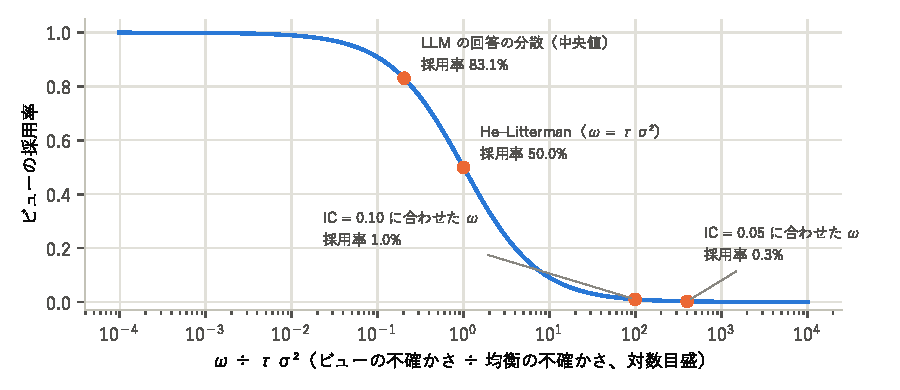
\includegraphics[width=0.92\linewidth]{fig_adoption_curve.pdf}
\caption{採用率と、2 つの不確かさの比の関係（式~\eqref{eq:adoption}）。点は、この資料で扱う設定。LLM の回答の分散は本プロジェクトのデータ（$\tau=0.025$、過去 1 年の日次の分散 $\sigma^2$ との比の中央値）。IC に合わせた $\omega$ は \chapref{ch:accuracy} の式~\eqref{eq:omega-ic} による。}
\label{fig:adoption}
\end{figure}

\figref{fig:adoption} から分かることを挙げる。

\begin{itemize}
\item He と Litterman の設定 $\omega=\tau\sigma^2$ では、採用率はちょうど 50\% である。ビューと均衡を同じ重みで扱う。
\item 本プロジェクトの LLM の回答の分散を $\omega$ に使うと、1 銘柄だけで見ても採用率は \V{llm.adopt.med}\% になる。複数の銘柄を同時に入れると、さらに高くなる（\chapref{ch:project}）。
\item 予想の当たり具合（IC）に合わせると、採用率は IC の 2 乗になる。IC が 0.05 なら 0.25\%、0.10 でも 1\% である。予想の当たり具合が現実的な水準なら、ビューはほとんど採用されないのが正しい。
\end{itemize}

採用率が 50\% と 1\% では、比率は大きく違う。$\Omega$ と $\tau$ を「なんとなく」決めると、結果の大半がその選び方で決まってしまう。これが、この資料の出発点である。

\section{大きさの感覚}\label{sec:scale}

$\tau\sigma^2$ と $\omega$ は、どちらも「期待リターンの不確かさ」の分散である。数字にしてみる。

\begin{exbox}[大きさの例（年率）]
株式の年率の標準偏差を $\sigma=20\%$ とすると、$\sigma^2=0.04$ である。$\tau=0.025$ なら $\tau\sigma^2=0.001$、その平方根は 3.2\% である。つまり事前分布は「期待リターンは均衡リターンのまわりに、標準偏差 3.2\% でばらつく」と言っている。

ビューの不確かさを、標準偏差で 3.2\% と置けば採用率は 50\%、10\% と置けば採用率は $0.001/(0.001+0.01)=9\%$、1\% と置けば 91\% である。「1 年後のリターンを ±1\% の精度で知っている」と言える投資家はいないので、91\% は信じすぎである。
\end{exbox}

単位にも注意がいる。日次・月次・年率のどれで書くかによって、$\sigma^2$ も $\omega$ も変わる。比 $\omega/(\tau\sigma^2)$ は、両方を同じ単位で書いていれば単位によらない。本プロジェクトのように「翌月の日次の平均リターン」を予想させる場合、$\Sigma$ は日次のリターンの共分散、$\omega$ も日次の平均リターンの分散でそろえる。元の実装では、日次のリターンから年率の金利を引いていた（『総合報告書』問題 5）。単位のずれは、採用率をそのまま狂わせる。

\section{調査メモの 4 つのファクターとの対応}

調査メモは、ビューと不確かさを作る材料を 4 つのファクターに分けている。この資料での扱いを\tabref{tab:factors}にまとめる。

\begin{table}[htbp]
\centering
\caption{調査メモのファクターと、この資料での扱い。}
\label{tab:factors}
\small
\begin{tabular}{p{1.8cm}p{4.2cm}p{5.0cm}p{1.4cm}}
\toprule
ファクター & ビュー $Q$ の作り方 & 不確かさ $\Omega$ の作り方 & 章 \\
\midrule
政治 & 地政学リスク・政策不確実性への感応度、シナリオ & 指数の水準で $\Omega$ を伸び縮みさせる（Han and Li 2023） & \ref{ch:politics} \\
テキスト・LLM & センチメント、LLM の予想（平均） & 回答のばらつき、確率の分布のエントロピー、複数のモデルの融合 & \ref{ch:text} \\
マクロ & 時系列モデル（EGARCH-M など）の予想 & 条件付き分散（Beach and Orlov 2007） & \ref{ch:macro} \\
財務・ESG & ファクターのプレミアム × 露出 & ファクターのプレミアムの推定誤差。ESG は共分散ではなく平均か制約で & \ref{ch:esg} \\
モメンタム & 過去のリターンの順位 & 予想の当たり具合（IC）、モメンタムのボラティリティ & \ref{ch:momentum} \\
\bottomrule
\end{tabular}
\end{table}

どのファクターでも、考えることは同じである。

\begin{enumerate}
\item ビューの値 $Q$ を、予想の当たり具合に見合った大きさにする（\chapref{ch:accuracy}）。
\item 不確かさ $\Omega$ を、実際の予想の誤差の大きさに合わせる。誤差の相関も入れる（\chapref{ch:accuracy}、\chapref{ch:project}）。
\item 最適化の段階で、ずれの大きさ（トラッキングエラー）に上限を置く（\chapref{ch:te}）。
\end{enumerate}

\begin{keybox}[この章のまとめ]
\begin{itemize}
\item BL で結果を大きく左右するのは $\tau$、$Q$、$\Omega$ の 3 つである。
\item 1 資産・1 ビューなら、均衡からビューへ動く割合（採用率）は $\tau\sigma^2/(\tau\sigma^2+\omega)$ である。
\item He--Litterman の設定では採用率は 50\%、予想の当たり具合に合わせると IC の 2 乗（多くは 1\% 未満）になる。この差が、BL の結果の差の大部分を生む。
\end{itemize}
\end{keybox}
